\documentclass{article}
\usepackage{graphicx} % Required for inserting images
\usepackage{wrapfig}
\usepackage{subcaption}
\usepackage{float}
\graphicspath{{./images/}}


\usepackage[backend=biber, style=apa, sorting=nyt]{biblatex}
\addbibresource[]{ref.bib}

\title{A study of Swords}
% \author{Thomas Lower}
\date{January 2024}

\begin{document}

\maketitle

\pagebreak

\tableofcontents

\pagebreak

\section{Introduction} \label{intro}
Action and Adventure is one of the largest Genre's within the Cinematic world in terms of Box Office return \parencite{3}. Furthermore, Adventure can be found in the top 3 of all major gaming platforms \parencite{4}. As such, it makes sense to analyse the core of these genres, weaponry. In this article, I intend to focus upon melee weaponry as I find that these offer a healthy balance between animation potential, efficiency to craft and creative possibility. Specifically, I intend to study the various versions of the sword, due to the well established symbolism associated with the various types of within the current media.

The idea of blades being able to invoke a specific view or feeling is well established within the media world, to the point where the mere concept of a sword and its apparent popularity within media is itself constructed by the media. Within historical times (I will largely be referring to the Medieval era), swords were pretty much exclusively wielded by kings and rulers because of the fact that they were exclusively tools for fighting and served no secondary purpose. Thus, they were extremely rare and more commonly symbolic rather than a common use tool which everyone would have known how to use.

Within this, it is my intention to establish a set of symbolisms that a given weapon can portray, and then use photography to successfully capture these symbolic features. Thus, allowing me to reproduce such work in Computer Graphics that would allow swords to contribute actively to the narrative, as a posed to being passive actors. This means I wish for swords to be able to contribute to a scene in their own right, without the outside influence of other factors such as a character or location. The weapon will, itself, be an actor within the scene which contributes to the narrative.

All swords can be broken down into 3 basic components:
\begin{list}{-}{}
    \item A sharp blade which will be used to strike against targets / parry incoming attacks. (see figure \ref{fig:SwordBlade}).
    \item An optional cross guard which blocks an incoming strike from hitting the hand of the wielder. Sometimes also referred to as a handguard or crossbar. (see figure \ref{fig:SwordCross}).
    \item A handle with a size relative to the size of the blade - in units of the size of the hand of a human. (see figure \ref{fig:SwordHandle}).
\end{list}

\begin{figure}[h]
    \centering
    \caption{Pictures of 3 different swords to illustrate their three basic parts.}
    \label{fig:PartsOfSwords}
    \begin{subfigure}{0.3\textwidth}
        \includegraphics[width=1\textwidth]{1HandLongswordBlade.jpg}
        \caption{The blade of a one-handed longsword.}
        \label{fig:SwordBlade}
    \end{subfigure}
    \begin{subfigure}{0.3\textwidth}
        \includegraphics[width=1\textwidth]{Saber3Handle.jpg}
        \caption{The golden crossbar of a saber.}
        \label{fig:SwordCross}
    \end{subfigure}
    \begin{subfigure}{0.3\textwidth}
        \includegraphics[width=1\textwidth]{OrnateShortswordHandle.jpg}
        \caption{The handle of an ornate shortsword.}
        \label{fig:SwordHandle}
    \end{subfigure}
\end{figure}

\subsection{The Blade}

The sword of the blade is probably the most crucial - as this is the offensive object of the weapon. The sword blade has multiple different versions with subtle differences.

The sword blade can feature one sharpened edge or two. The two-sided blade offers an obvious offensive advantage because of the added flexibility of its attack. But, this must be balanced with the idea that the blade will therefore require double the maintenance to ensure the blade is properly sharpened, as well as also requiring the blade to be wider. When an object cuts, it uses the sharpened section of the blade to initially separate the object. The width of the blade is then used to push the two new parts further apart and ensure a full cut. This then maximizes blood loss and therefore damage to the target. The effect of blood loss can then be exemplified by placing a small slit in the centre of the blade for blood to run down (see figure \ref{fig:swordSlit}). 

\begin{figure}[h]
    \centering
    \caption{}
    \begin{subfigure}{0.49\textwidth}
        \includegraphics[width=\textwidth]{SaberDamagedBlade1.jpg}
        \caption{A closeup of the blade showing a crease where the rising parts of the blade meet.}
        \label{fig:SwordCrease}
    \end{subfigure}
    \begin{subfigure}{0.49\textwidth}
        \includegraphics[width=\textwidth]{SpearSide.jpg}
        \caption{The side of a spear to show the slope effect.}
        \label{fig:SpearSide}
    \end{subfigure}
    \begin{subfigure}{\textwidth}
        \centering
        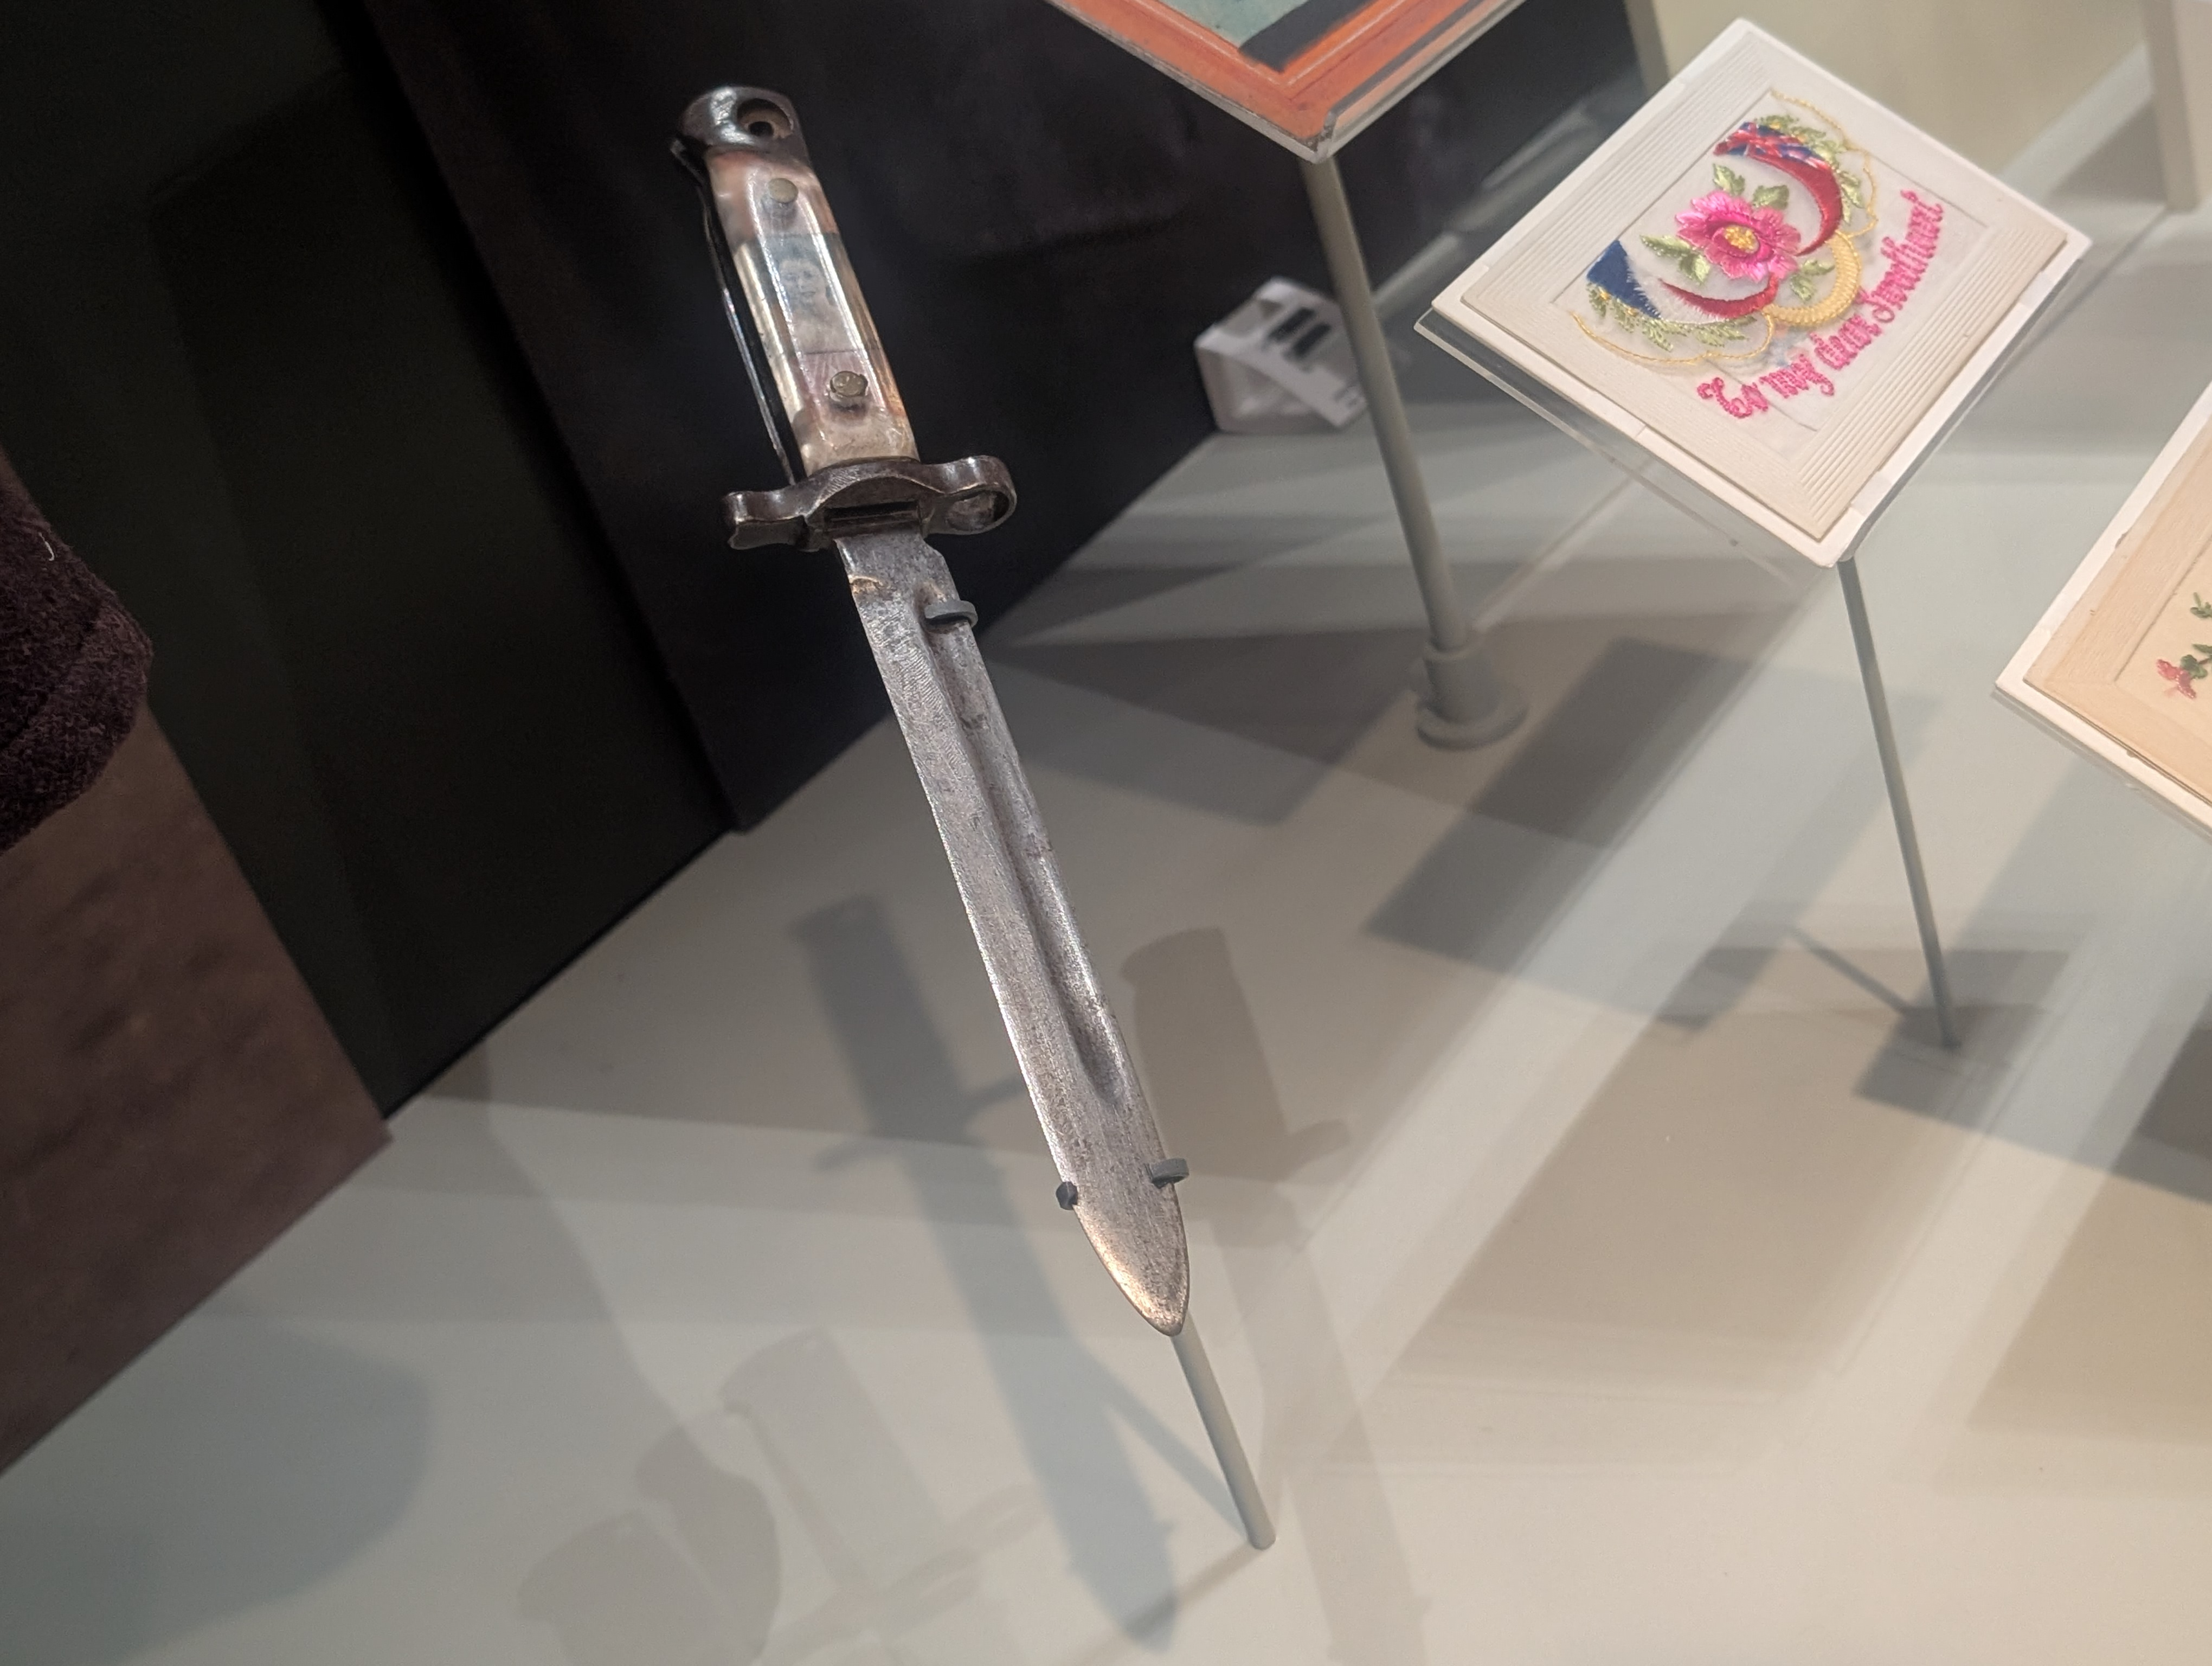
\includegraphics[width=0.5\textwidth]{Dagger2.jpg}
        \caption{A dagger with a slit through which blood can run after stabbing a person to enable a person to more effectively bleed out without having to remove the knife.}
        \label{fig:swordSlit}
    \end{subfigure}
\end{figure}

However, this requires the width of the blade to increase at a certain rate as too high an increase will negatively affect the speed of the blade and its ability to cut effectively (try to imagine the different between cutting with a sharp edge, and cutting with the face of a cube (see this effect in figure \ref{fig:SpearSide})). It is because of this that the blade therefore becomes much wider if having multiple sharp edges which would have put a strain on materials with which these tools would be forged. It would have also been a heavier weapon if having multiple blades which, in turn, would therefore become more difficult to wield. This issue can be seen in figure \ref{fig:WideDagger}

\begin{figure}[h]
    \centering
    \includegraphics[width=0.25\textwidth]{LargeBladeDagger.jpg}
    \caption{A Dagger with a wide blade due to its double handedness.}
    \label{fig:WideDagger}
\end{figure}

Another consideration of the number of sharpened edges is the famous "crossed blades" moment in a filmed fight scene. In this, 2 characters wielding longswords will become very close and hold their swords against each other - each pressing the blade against each other in an attempt to simply overpower their opponent. During this situation, a combatant would have a clear advantage if they are able to apply pressure to the back of the blade as Archimedes' research on levering would imply that this is a much more effective place to give force to overpower their opponent \parencite{bunn2017archimedes}. This, however, would only be possible on a single edged sword as otherwise the attacker would almost definitely slice their own hand open if they were to press on the other bladed side of a 2 sided blade.

The point of the blade is also of valid importance as some blades will focus towards a singular spike at the edge, while others will fail to do so. The spike at the end opens the blade up to an additional straight - piercing - strike. This strike is much faster and - due to the lack of angular attack - is much more difficult to parry. However, comes at the cost that the bladed edge close to this point becomes somewhat less effective. Above, I mentioned the width of the blade providing an effective method of properly separating the parts of the target which were cut. If the blade focusses into a point though, this width will have to shrink down towards the end of the blade to allow it to form a point, which renders the bladed edge less effective as it loses this separating ability.

\subsection{The Guard}
The guard of a weapon is an incredibly useful part to the sword, from the perspectives of both the fighter and the artist. The handguard or crossguard (either wording is acceptable), from a fighting standpoint, provides an exceptional and simple protection while fighting. Due to the shape of the blade, it is not uncommon for a strike to slide down the blade, towards the handle. With nothing to protect the defender, their fingers would easily see damage. Or at the very least, they would be disarmed with great ease. This is obviously a massive disadvantage, therefore, it became incredibly common for swords (especially shorter variants such as the shortsword and rapier) to feature a crossguard or handguard to protect the wielder.

\begin{figure}[H]
    \centering
    \caption{A collection of crossguards from various blades}
    \label{fig:Crossguards}
    \begin{subfigure}{0.3\textwidth}
        \centering
        \includegraphics[width=\textwidth]{cross6.jpg}
        \caption{The crossbar of a sabre.}
        \label{fig:Cross1}
    \end{subfigure}
        \begin{subfigure}{0.3\textwidth}
        \centering
        \includegraphics[width=\textwidth]{cross2.jpg}
        \caption{The crossbars of 2 rapiers.}
        \label{fig:Cross2}
    \end{subfigure}
        \begin{subfigure}{0.3\textwidth}
        \centering
        \includegraphics[width=\textwidth]{cross3.jpg}
        \caption{The crossbar and basic handguard of a sabre.}
        \label{fig:Cross3}
    \end{subfigure}
        \begin{subfigure}{0.3\textwidth}
        \centering
        \includegraphics[width=\textwidth]{cross4.jpg}
        \caption{The crossbar and handguard of a sabre.}
        \label{fig:Cross4}
    \end{subfigure}
        \begin{subfigure}{0.3\textwidth}
        \centering
        \includegraphics[width=\textwidth]{cross5.jpg}
        \caption{The crossbar of a dagger.}
        \label{fig:Cross5}
    \end{subfigure}
        \begin{subfigure}{0.3\textwidth}
        \centering
        \includegraphics[width=\textwidth]{cross1.jpg}
        \caption{The crossbar of a longsword.}
        \label{fig:Cross6}
    \end{subfigure}
\end{figure}

It is noteworthy that the crossguards of blades is usually quite thin and small, this feature gave rise to a specific form of artistic expression. It became entirely possible for unique and interesting patterns to be created and placed in position to act as a handguard or crossguard. This enables weapons to display certain specific concepts - usually regality as this art form would have been expensive to craft. Therefore, requiring the wealth of a lord or monarch. Examples of these items can be seen in figure \ref{fig:crossguardsAdvanced}

\begin{figure}[H]
    \centering
    \caption{A collection of artistically designed crossbars and handguards.}
    \label{fig:crossguardsAdvanced}
    \begin{subfigure}{0.3\textwidth}
        \centering
        \includegraphics[width=\textwidth]{cross2.1.jpg}
        \caption{The circular crossbar of a rapier with patterns engraved into the metal.}
        \label{fig:Cross2.1}
    \end{subfigure}
        \begin{subfigure}{0.3\textwidth}
        \centering
        \includegraphics[width=\textwidth]{cross2.2.jpg}
        \caption{A rapier with a fencing style conic handguard.}
        \label{fig:Cross2.2}
    \end{subfigure}
        \begin{subfigure}{0.3\textwidth}
        \centering
        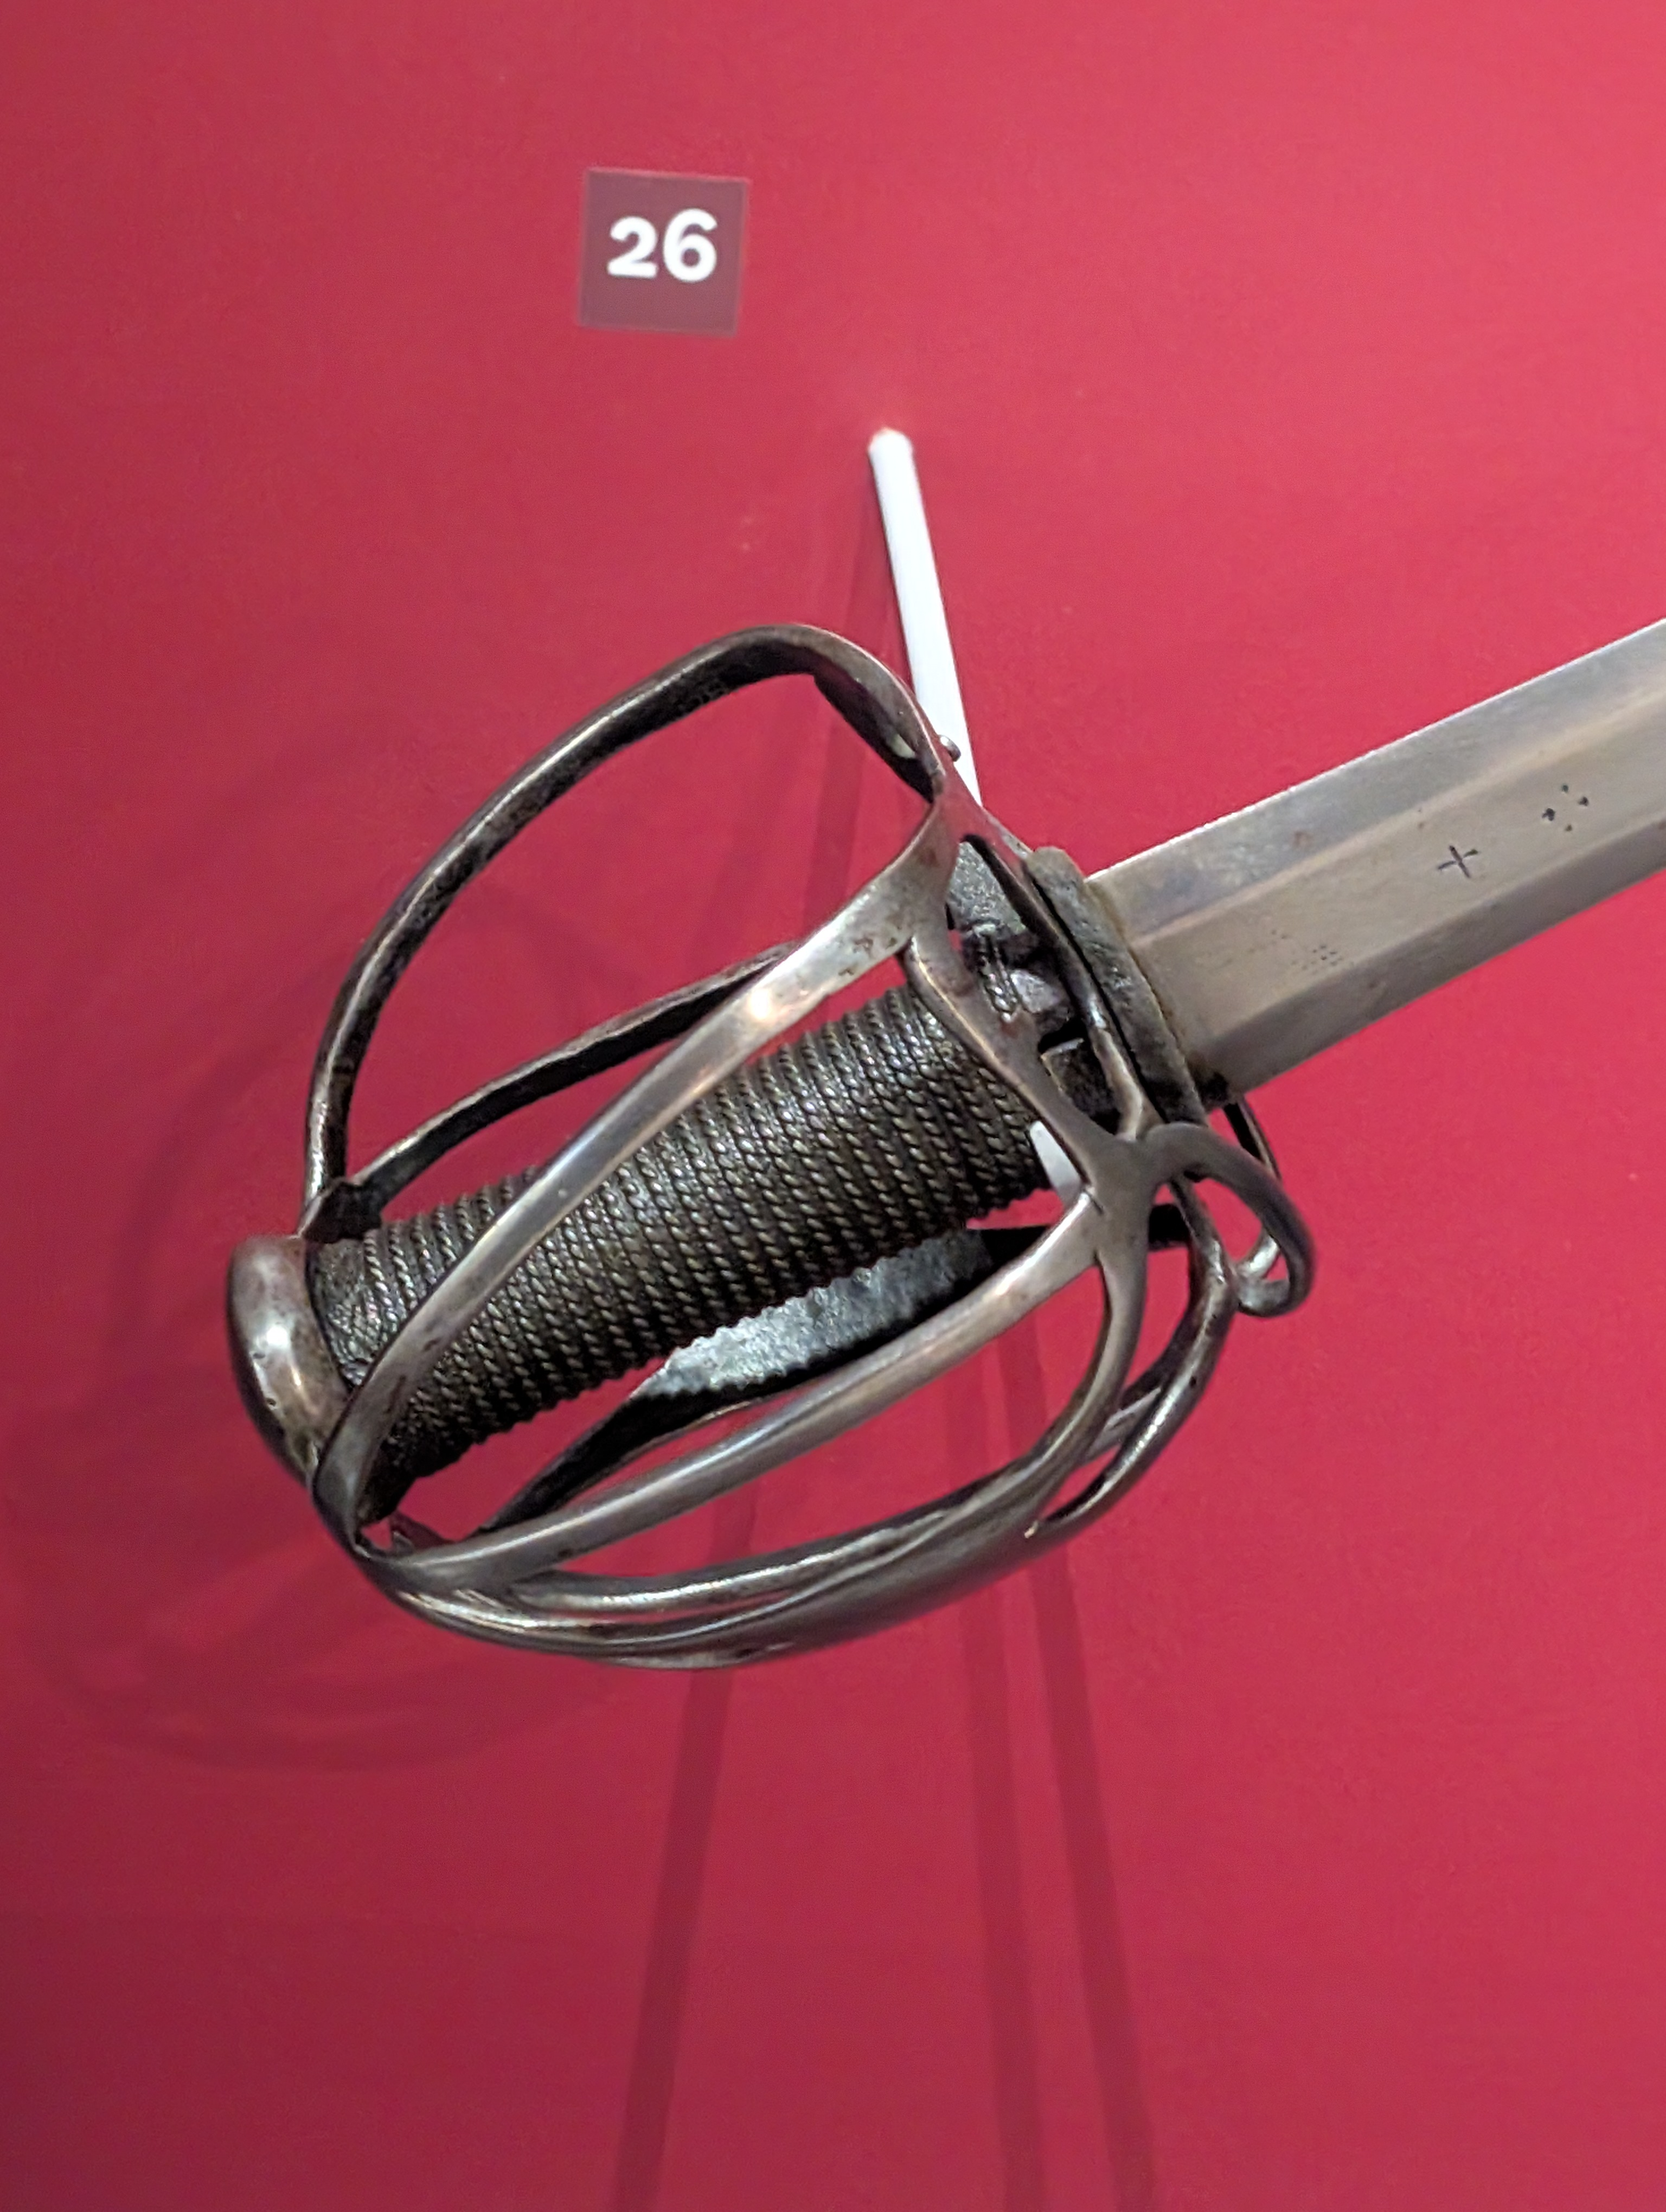
\includegraphics[width=\textwidth]{cross2.4.jpg}
        \caption{A sabre with a basic spindly handguard which would only protect against slashing harm.}
        \label{fig:Cross2.4}
    \end{subfigure}
        \begin{subfigure}{0.75\textwidth}
        \centering
        \includegraphics[width=\textwidth]{cross2.3.jpg}
        \caption{A collection of crossguards for Japanese katanas. For these weapons, the guard was a separate object that was placed over the blade and could be switched in and out.}
        \label{fig:Cross2.3}
    \end{subfigure}
\end{figure}

\pagebreak

\section{Swords in the media} \label{media}
As mentioned in section \ref{intro}, Films and Video Games that feature melee weaponry are often some of the most popular. Here I will go over a few and their use of these weapons:

\subsection{For Honor}
(\fullcite{forhonor}).
For Honor is a multiplayer fighting game known for its mechanics around stances, allowing any character to hold their weapon in one of three possible stances. An important thing to note for this game is the idea that the weapons are specific to a character - a character who supposedly has specific training, holds specific armour and has specific abilities. This, therefore, implies that these weapons are a part of the characters identity and representation the same as any other aspect. This then presents the idea that weaponry is capable of expressing a specific idea or symbolism, an idea that is found throughout other media.

\subsection{The Elder Scrolls V: Skyrim}
\begin{wrapfigure}{r}{0.25\textwidth}
    \centering
    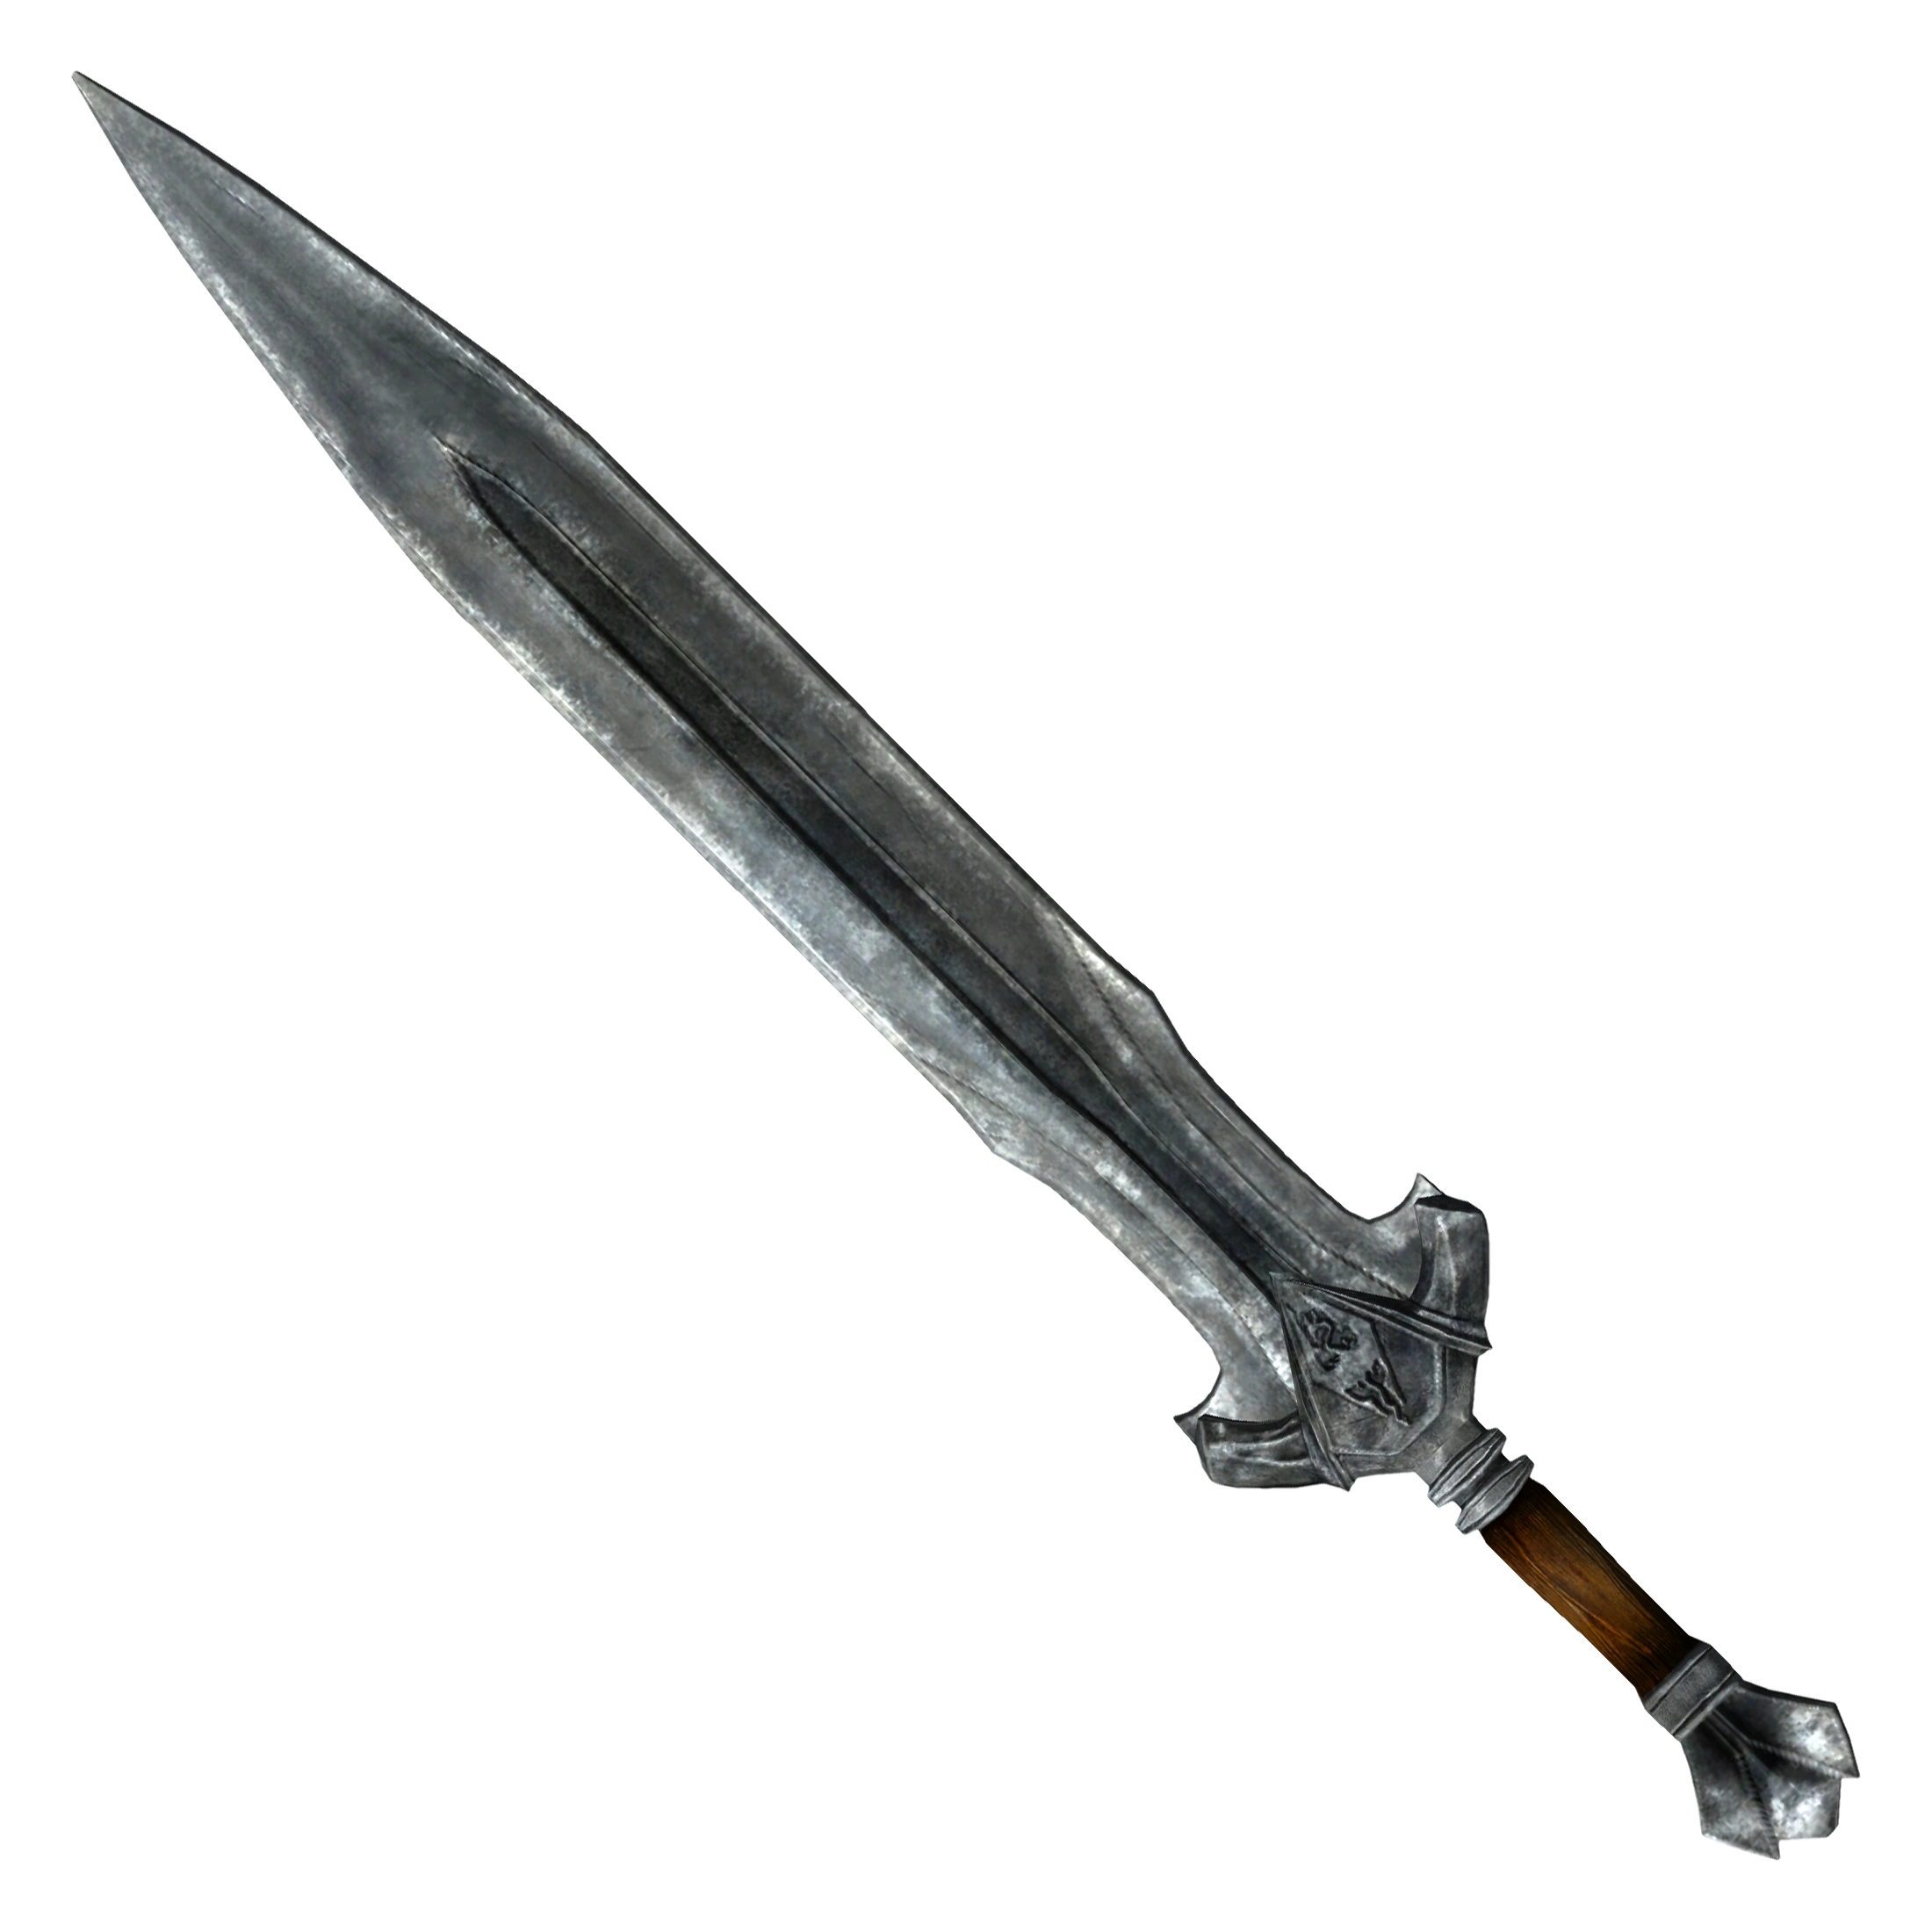
\includegraphics[width=0.25\textwidth]{ImperialSword.png}
    \caption{\parencite{imperialSword} An Imperial Sword from the game "Skyrim".
    }
    \label{fig:ImperialSword}
\end{wrapfigure}
(\fullcite{skyrim}).
Skyrim is a Role Playing Game set in a fantasy setting of its namesake - within the world of Tamreil. This game features multiple different types of sword including the sword, longsword and greatsword. However, I feel the most important to note is the first sword encountered by the player in the game - the Imperial sword. At the beginning of the game, the player is given a choice to join either the imperial legion or the stormcloak rebellion. The given weapon of the stormcloaks is an axe - typically associated with Viking culture and a brutish mentality which then helps to contrast against the weapon given by joining the imperials, which then helps to give an impression of legality and structure. Such being the common representation of the sword.

\subsection{The Lord of the Rings}

(\fullcite{lotr}).
The Lord of the Rings is both a book and film series set in a medieval fantasy world. Being the generic conventions of the fantasy genre, these feature many different types of swords and blades. The most notable being the dagger held by Bilbo - one of the few magical weapons in the series (to be expected of a dagger as stated in section \ref{daggerSymbol}) as well as the longsword held by Aragorn (which brings its many associations to his own character identity set out in section \ref{longswordSymbol}).

\begin{figure}[h]
    \centering
    \caption{\parencite{Sting} The blade "Sting" from the film "The Hobbit" glowing in the presence of orcs.}
    \label{fig:Sting}
    \includegraphics[width=0.5\textwidth]{Sting.png}
\end{figure}

\subsection{Pirates of the Caribbean}

(\fullcite{potc})
The Pirates of the Caribbean is a film series following the exploits of pirate Jack Sparrow and the other pirates and sailors he encounters on his journeys. These feature 2 main types of sword, the sabre and rapier. There is a running joke within the series that concerns a particular sword: A rapier produced by the character William Turner for the Commodore James Norrington. The joke runs that anyone who sees the sword and has a chance to examine it states "nice sword" before taking it. This aligns with the representation of the rapier being an example of regality, as stated in section \ref{rapierSymbol}.

\begin{figure}[h]
    \centering
    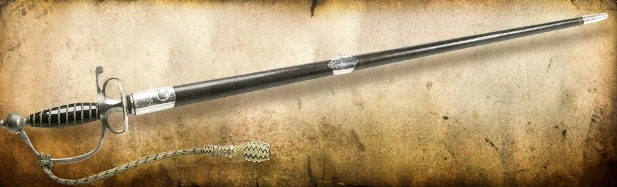
\includegraphics[width=0.8\textwidth]{Norringtonssword.png}
    \caption{\parencite{potcsword}The "nice sword" crafted by William Turner for Commodore James Norrington}
    \label{fig:potcSword}
\end{figure}

\subsection{How I met your Mother}

(\fullcite{himym})
The show how I met your mother is comedy series in which the protagonist Ted Mosby tells the story of how he met his mother to his children. The comedy series may appear to be a strange choice for this, however, this show features 2 sabres which are decorative items hung on the wall of their flat. This fits the general symbolic association of the sabre, that it is a largely decorative piece (see more in section \ref{saberSymbol}). However, in the Season 1, Episode 8, entitled "The Duel", Ted and his friend Marshall actually use these swords to duel \parencite{theduel}, such that they fulfil Chekhov's Gun \parencite{delaney1990chekhov} and allow these weapons to generate their own symbolism through their use, that of their own friendship.

\subsection{Ghostrunner}

(\fullcite{ghostrunner})
Ghostrunner is a fast-paced game in which a cyborg wielding a katana must run through a cyberpunk city while slashing at enemies with guns. This game is an expert at presenting the katana and showing its intended use. The concept of the katana is that it can be swung fast and allows for quick movement - almost a merge between the rapier and the longsword. Although it is worth noting that this representation from Ghostrunner is largely due to the way that the weapon is wielded and used in the game, rather than its design and structure. However, recognising this is still useful for the establishment of a base case, from which my own research can build from.

\subsection{Ahsoka}

(\fullcite{ahsoka})
Ahsoka was a series set in the marvel universe, following the journey of Ahsoka Tano after the events of order 66. The character of Ahsoka can be seen to hold 2 separate types of lighsaber - which each have a comparable type of sword. In 1 hand she holds what is referred to as a "shinto-blade", a lightsaber equivalent of a shortsword. As well as a normal lightsaber, the equivalent of a longsword. She holds an extremely acrobatic style of fighting with these 2, allowing herself to act more defensively from 1 hand and more offensively from the other. Overall, balancing the drawbacks of 1 blade with the positives of another. 

The show also features an antagonist named Baylan Skoll. This character wields a large lightsaber which is treated with the same fighting style of a greatsword. This contrast of Ahsoka's agility against this type of weapon is excellent at displaying the various representations of weapons as Ashoka uses short quick attacks while dodging out of the way of Baylan's strong attacks while he himself blocks Ahsoka's own attacks.

\pagebreak

\section{Sword Symbolism} \label{swordSymbol}
As discussed prior, the term sword is in fact a category to describe many different types of weapons \parencite{furat1998brief}, all of which follow the same general shape pattern of: handle → hand guard → single, continuous blade.
All swords would feature a common representation: that of honour. Within history, most combat would be achieved through armies of levies, who were donated troops from the barons of a kingdom. These troops would not be outfitted by the monarch, but rather, they would outfit themselves with whatever weaponry they could find. Be it scythes, hoes, hatchets or pikes. It would be extremely rare for them to equip a sword as this weapon has no other purpose other than fighting. Thus, it would make no sense for a peasant levy to own a sword. The only people who would battle with swords would be the monarchs and knights of the army; they would be able to afford a sword as well as afford the time to train with it. This is what causes the sword to be commonly associated with honour, as the monarch was \textit{theoretically} the most honourable soldier in the army. Furthermore, this also allows them to serve as a symbol of hope. While the monarch was alive, it could be assumed that you were still winning - or at the very least not losing - the battle. Therefore, if you could see a sword, then you could see your monarch, and you were probably winning.

\subsection{Short sword} \label{shortSwordSymbol}
One of the most basic types of sword, would be more accurately described as a short sword \parencite{mcnab2010swords}. This weapon features a short blade length of no more than 30 cm and often lacks a proper handguard. Thus giving it a sense of aggression as it lacks this key protective implement, requiring the wielder to rely on pure offence in order to overpower their enemies as a posed to being able to fall back to a defensive position when needed. It also requires extreme close range to the target in order to be used effectively, therefore requiring the person holding this weapon to be within direct shot of blood and other gut-like objects when released from the body with this weapon. This creates an association with it being bloody and brutal as the attacker must be willing to become covered in their enemies blood. Thus, the weapon can be considered bloody and aggressive.

\begin{figure}[h]
    \centering
    \caption{A collection of shortswords being used in brutish circumstances}
    \begin{subfigure}{0.3\textwidth}
        \includegraphics[width=\textwidth]{SwordToKillChild2.jpg}
        \caption{A shortsword used when a king threatened to split an infant in half when 2 mothers claimed maternity over the child.}
        \label{fig:killChild}
    \end{subfigure}
    \begin{subfigure}{0.3\textwidth}
        \includegraphics[width=\textwidth]{DavidShortsword.jpg}
        \caption{The shortsword held by David while standing on the decapitated head of Goliath.}
        \label{fig:goliathDead}
    \end{subfigure}
    \label{fig:shortswords}
\end{figure}

\begin{figure}[H]
    \centering
    \includegraphics[width=0.3\textwidth]{NewVSOldTestament.jpg}
    \caption{2 Stained glass windows depicting the Old Testament (bottom) and New Testament (top).}
    \label{fig:shortswordsTestament}
\end{figure}

In figure \ref{fig:shortswordsTestament}, these stained-glass windows assist to illustrate the point of the vicious representation of the shortsword. The top of the two stained-glass windows is representative of a scene from the New Testament of the bible, while the bottom is of the Old Testament. There is a general understanding in critical analysis (\parencite{fretheim2004god}, \parencite{lilly2012war}, \parencite{creach2016violence}) that the Old Testament of the bible is much more violent than that of the New Testament. The presence of the short sword within the bottom window certainly helps to convey this as this weapon is commonly associated with the violent and the bloody. Thus, the inclusion of this in the image helps to portray the contrast in violent tendencies between the old and new testaments.

\subsection{Dagger} \label{daggerSymbol}
This contrasts greatly to the dagger which would be considered sly and agile. The symbolism related to such a weapon is often that of deceit and mistrust. This is due to its small size and the fact that this allows it to play a crucial part in assassinations. This is true of the real world, such as the death of Julius Caesar \parencite{caesar} in which a character can be seen holding a dagger. As well as in fictional pieces such as Macbeth in which the character Macbeth famously asks: \begin{quote}
    "Is this a dagger I see before me?"
\end{quote}
before stabbing King Duncan \parencite{macbeth}. Therefore, daggers are often associated with evil as they bring about deceitful death against powerful people.

\begin{figure}[h]
    \centering
    \includegraphics[width=0.5\textwidth]{PersiusWithDagger.jpg}
    \caption{A dagger held by Persius after he slayed Medusa.}
    \label{fig:PersiusDagger}
\end{figure}

Daggers also have a second association, that of the occult. Due to the ease of secrecy as well as the precision - because of the size of the blade - this weapon is often associated with cult-like rituals that require a donation of blood or other sacrifice. The precision of a dagger allows a participant of such a ritual to control the amount of blood used, such that their life is not at risk from blood loss if it is not supposed to be. This association with brutish occult methods is further enhanced because of the need for the wielder to become very close to their target. This, essentially, makes it impossible for a person to avoid getting the blood and innards of the target on themselves, thus requiring a strong constitution or even appreciation of these otherwise disgusting fluids. Thus leading an association with the occult as those who would practice such rituals are often associated to a lack of remorse around the inner parts and guts of others.

\subsection{Longsword} \label{longswordSymbol}
Both of these weapons would be considered to be aggressive, demonstrating the lethality of swords. To search for the representation of honour and protection, one must seek the longsword or broadsword. This weapon features a much longer blade, such that to support it properly would require a 2 handed grip, but could still be wielded with one hand if necessary. As well as being featured with a handguard. The size of this weapon allows it to more effectively parry and block, thus allowing it to present as more well-rounded in comparison to the weapons found in sections \ref{daggerSymbol} and \ref{shortSwordSymbol}, being capable of slashing at an enemy as well as blocking an attack. This leads to it being the symbol on many coats of arms such as London \parencite{fox1894book} and New York state \parencite{newyorkflag} as it represents adaptability and strength. Both traits being desirable for a group to associate themselves with.

\subsection{Sabre} \label{saberSymbol}
The sabre is an important weapon when considering symbolism as it is almost exclusively used as a symbolic artefact rather than a military tool. The design of the sabre follows the curved fashion of the Japanese katana, however, with two key differences. The katana stills merges to a single point at the end that is capable of piercing, while the sabre curves round to form a shape not dissimilar to that of a banana. Furthermore, the katana is sharpened while the sabre is usually square at its edges (at least in modern day) to avoid a person accidentally harming themselves on the weapon, due to it being largely a decorative piece.

Its symbolism is exclusively that of honour and rank. Specifically the honour that could be associated with that of a high ranking general or other military leader as they would be those who are awarded such an item. This explains why many sabres often feature ornate handguards and handles, as well as writing inscribed upon the blades of the swords.

\begin{figure}[H]
\centering
\caption{A collection of images from sabres at the National Army Museum.}
\label{fig:sabreImages}
\begin{subfigure}{0.3\textwidth}
    \includegraphics[width=\textwidth]{Saber4Blade.jpg}
    \caption{An ornate golden sabre with a long inscription.}
    \label{fig:Saber4}
\end{subfigure}
\begin{subfigure}{0.3\textwidth}
    \includegraphics[width=\textwidth]{Saber5.jpg}
    \caption{A military sabre.}
    \label{fig:Saber5}
\end{subfigure}
\begin{subfigure}{0.3\textwidth}
    \includegraphics[width=\textwidth]{Saber6.jpg}
    \caption{An silver sabre with an engraving along the blade.}
    \label{fig:Saber6}
\end{subfigure}
\begin{subfigure}{0.3\textwidth}
    \includegraphics[width=\textwidth]{Saber2.jpg}
    \caption{A light cavalry troopers sword featuring a sharkskin handle.}
    \label{fig:Saber2}
\end{subfigure}
\begin{subfigure}{0.3\textwidth}
    \includegraphics[width=\textwidth]{Saber3.jpg}
    \caption{An infantry hanger sword given to all privates until 1768.}
    \label{fig:Saber3}
\end{subfigure}
\end{figure}

\subsection{Rapier} \label{rapierSymbol}
Now we can begin to discuss more specialized weapons. To begin, lets start with a personal favourite of mine, the rapier. This sword is also commonly referred to as a fencing sword and is characterized by an extremely thin blade - such that it may flop and bend under movement of the handle. It also often features a rounded guard or set of rings that covers the hand or fingers \parencite{walker2002rapier12}. This sword acts as a symbol for one very specific concept, elegance. The rapier is not a slashing weapon like most swords, but rather, exclusively a piercing weapon \parencite{walker2002rapierNoCut}. Such that it uses straight stabs to cause damage to an individual. These straight stabs are designed to be done extremely quickly in extremely precise spots. To wield this weapon therefore requires both attention and intelligence - to know when and where exactly to stab. These requirements lead to the weapon becoming a dedication for its wielders as only somebody who is specifically trained with this weapon will be able to use it properly, anyone else will struggle. With this dedication, a certain grace and elegance follows, in both the biological and mathematical knowledge \parencite{walker2002rapier25} to know where to stab, and the form and positioning that is required to stab swiftly and effectively. Furthermore, This weapon is exclusively offensive as the flimsy of the blade offers no possible defence. However, its lack of weight offers a different approach. With a lightweight weapon that bends to allow easy aerodynamics, plus the wielder needing to hold the correct form to allow extremely fast movements for stabs, this weapon lends itself well to the agile. This massively supports the idea of elegance as the agility often results in movements that can be quite shocking and interesting to the eye as a wielder dodges and weaves about heavier and less manoeuvrable types of blade.

The association with elegance also originates from its association with the ruling elite, all of whom would wear this weapon as a part of their civil attire - especially in France and Germany within the Middle Ages \parencite{correa2013history}. The simple fact that all of these people would be commonly carrying this weapon led to a strong association with that of elegance as the elegance of the ruling classes became intrinsically attached to the items they carried. This also leads to the more practical symbolism of the rapier - which is that of regal influence and upper class status.

\subsection{Greatsword} \label{greatswordSymbol}
Another important weapon to consider is the greatsword or claymore. This weapon is known exclusively for its massive size. Requiring a minimum of 2 hands to even hope to lift it properly. However, this is not enough in most cases. To lift a claymore would, similar to the rapier, require a large amount of training in order to wield it properly. This weapon perhaps offers the opposite symbolism to the rapier. Where the rapier was a symbol of intelligence and agility, where the wielder only needed to pay attention to their own strikes and dodge the enemies. The claymore relies on sheer brutish strength, and timing strikes and swings with the opponent in order to counteract its complete lack of manoeuvrability (bearing in mind that this weapon is often dragged along the ground as its sheer weight is too much to be carried normally). This ultimately leads to an association with strength, but not the same brutish strength that short swords were known for. No, this is an aged and experienced strength, the strength that comes with training and dedication. A strength mixed with awareness and timing, such that the lack of agility of the blade poses no real issue. This practice also leads to a more practical symbolism of the greatsword in the form of age and wisdom - something comparable to the staff of a wizard - due to the practice required by the wielder to achieve strong timing.

It is also worth noting the aggression associated with this weapon, in some part, simply due to its sheer size. But also due to the practice of wielding this weapon. To wield this weapon properly, any movement with the blade should be considered as an attack as the momentum needed for an attack is the only possibility for the wielder to move the weapon effectively.

\pagebreak

\section{Iterations of Sword Symbolism photography}

\subsection{Iteration 1} \label{Iteration1}

\begin{figure}[h]
    \centering
    \caption{}
    \label{fig:Iteration1}
    \begin{subfigure}{0.49\textwidth}
        \includegraphics[width=1\textwidth]{Iteration1.1.jpg}
        \caption{}
        \label{fig:Iteration1.1}
    \end{subfigure}
    \begin{subfigure}{0.49\textwidth}
        \includegraphics[width=1\textwidth]{Iteration1.2.jpg}
        \caption{}
        \label{fig:Iteration1.2}
    \end{subfigure}
\end{figure}

The first 2 blades featured in figures \ref{fig:Iteration1.1} and \ref{fig:Iteration1.2} features a dull, steel-like metal blade with 2 sharp edges, a basic circular hand guard and an uninteresting handle. These weapons are not being held in any way. As a result, these blades are rather unimpressive such that they fail to convey any particular element of story or narrative - such being my final goal. The only characteristic these blades could be said to have is a slight damage to the blade, suggesting age or lack of care. However, this lack of interesting characteristics could be considered to be characteristic in and of itself. Allowing the blade to present itself as being standard or unimportant could be useful metaphorical representations of war and conflict, or maybe in representation of the soldiers who may have wielded these weapons. Nonetheless, these symbolisms would require further factors outside of the weapon itself and its direct use in order to be imagined, thus the blade is unable to present a narrative or function as a narrative device. To improve, the blades should feature some form of interesting shape, colouring or iconography. Furthermore, the blade could be held in an interesting pose or stance, such that an obvious emotion or state could be drawn from it.

\pagebreak

\subsection{Iteration 2} \label{Iteration2}

\begin{figure}[h]
    \centering
    \caption{}
    \label{fig:Iteration2}
    \begin{subfigure}{0.49\textwidth}
        \includegraphics[width=1\textwidth]{Iteration2.1.jpg}
        \caption{}
        \label{fig:Iteration2.1}
    \end{subfigure}
    \begin{subfigure}{0.49\textwidth}
        \includegraphics[width=1\textwidth]{Iteration2.2.jpg}
        \caption{}
        \label{fig:Iteration2.2}
    \end{subfigure}
\end{figure}

The figures \ref{fig:Iteration2.1} and \ref{fig:Iteration2.2} is arguably the inverse of the iteration in section \ref{Iteration1} in terms of the presence of iconography and colouring. The entire blade features a stark contract between gold and black. The blade features a dragon as a cross guard and a lions head on the end of the handle. There is also a paragraph of inscription on the blade as well as many pieces of iconographic art decorating the blade. All of which creates an overwhelmingly regal appearance. It is obvious that this weapon was never meant to be used in battle, rather it is simply a display piece. This is one of my issues with it. Chekhov's Gun \parencite{delaney1990chekhov} suggests that a gun featured in a scene should be fired. Thus, it follows that a sword in a scene must be used in a battle. This blade not being able to be used in battle would therefore limit its narrative potential to an extreme level as it is unable to be used in a battle, and therefore cannot actively contribute to the narrative, only passively. My goal being weapons that can be used to add to the narrative in their own right, requires weapons that can, in fact, add to the scene. A weapon that cannot be swung will not add to the scene and thus this iteration must be improved upon.

Furthermore, I feel that while the elaborate design is successful in adding a regal element to the blade, it is simply too much. The dragon and lion plus the paragraph plus the patterns on the blade is simply too much. It overwhelms the eye which in turn, would cause it to be less effective at conveying narrative in animation - a visual medium.

Overall, what can be learned from this iteration is that the weapon must appear actively useful for fighting and combat, as well not being too visually overwhelming. It must be sensible in its design while still being interesting.

\pagebreak

\subsection{Iteration 3} \label{Iteration3}

\begin{figure}[h]
    \centering
    \caption{}
    \label{fig:Iteration3}
    \begin{subfigure}{0.49\textwidth}
        \includegraphics[width=1\textwidth]{Iteration3.1.jpg}
        \caption{}
        \label{fig:Iteration3.1}
    \end{subfigure}
    \begin{subfigure}{0.49\textwidth}
        \includegraphics[width=1\textwidth]{Iteration3.2.jpg}
        \caption{}
        \label{fig:Iteration3.2}
    \end{subfigure}
\end{figure}

Figures \ref{fig:Iteration3.1} and \ref{fig:Iteration3.2} are much closer to achieving my goals. The first of the two shows a handguard with an interesting shape that adds character to the blade without overwhelming it. Furthermore, the colour damage to the handguard allows it to blend well with the handle and blade, such that all components follow the same theme - allowing them to further conform to a concept.

The blade itself features damage to the shape, allowing the silhouette to be effected, this is probably the most obvious narrative element of the blade, showing age and use. The colouration of the blade is also additive to the overall narrative appeal of the weapon as its damage furthers the concept of age and well use.

Overrall, the blade is very good at displaying a narrative concept within its own right. In a real use case, the weapon would likely see posing and usage to allow it to fulfil the prophecy of Chekhov's Gun \parencite{delaney1990chekhov}, however, this would also require features outside of the weapon itself. Thus for these purposes, the weapon is fine at displaying the capacity for a sword to convey a story.

\pagebreak

\subsection{Iteration 4} \label{Iteration4}

\begin{figure}[h]
    \centering
    \caption{}
    \label{fig:Iteration4}
    \begin{subfigure}{0.49\textwidth}
        \includegraphics[width=1\textwidth]{Iteration4.1.jpg}
        \caption{}
        \label{fig:Iteration4.1}
    \end{subfigure}
    \begin{subfigure}{0.49\textwidth}
        \includegraphics[width=1\textwidth]{Iteration4.2.jpg}
        \caption{}
        \label{fig:Iteration4.2}
    \end{subfigure}
\end{figure}

The images in figure \ref{fig:Iteration4} are from 2 separate stone carvings. Figure \ref{fig:Iteration4.1} is from a larger than life statue (around 9 feet tall) while figure \ref{fig:Iteration4.2} is a minifigure in a nativity-esque crucifixion scene. Both figures feature the framed characters holding longswords with the blade against the ground. The longsword remains in its scabbard rather than being unsheathed. At first glance this feature may appear to subtract from their narrative potential as they are clearly not about to be used. However, I believe the fact that they are both being held by a character (both slanting slightly to the left) would in fact allow itself to create a separate narrative concept. The fact that the blade is being held means it does not lack the effects of Chekhov's Gun \parencite{delaney1990chekhov} as it is still being used in an active situation (even if not being fought with, it is an active element in the scene). Keeping it in the scabbard would allow it to present the idea of potential, the mystery acting as a hermeneutic code \parencite{barthes1972semiotics} which is an advanced narrative technique to keep an audience interested in the potential of a narrative by obscuring information. The reason I believe this would work just as well as if the sword were to be used in a combat scenario is due to the fact that Barthes also defines an "action code" which would have the same effect of attracting and engaging an audience, but using an action rather than the mystery of its potential.

Another strong feature of this iteration is the use of the various associations of the longsword (more info about this available in \ref{longswordSymbol}). The longsword holds a symbolism of honour and strength. Thus, the sword being wielded by a religious figure or knight in the presence of Christ would contribute greatly to the overall intention of the sculptures (such intention being to imply the strength and power of Christ). Because of this association with honour and strength, the longsword holds a second representation of goodness, such which is obviously used by these pieces to further enhance their own representation. The fact that these stand-alone pieces of art are using weapons in the same ways that I have described previously to present this representation and interpretation is immensely powerful and important for helping to prove my goal of allowing weapons to contribute to a narrative in ways other than simply slicing and damaging opponents.

The only downside of these pieces is that they are indeed carved from stone rather than forged of metal. Thus meaning that they are struggling to inform the creation of materials to provide narrative clarity. However, other iterations (mainly section \ref{Iteration2}) more than compensate for this, providing information to help rectify this otherwise singular lacking in this iteration.

Overall I feel that this iteration is incredibly strong despite its lack of material diversity, as it shows the generic symbolism of the chosen weapon in action, allowing it to clearly present the concepts associated with it. Furthermore, it works with advanced narrative theories to help build its narrative strength. Overall, creating a rather useful example to demonstrate the ability of blades to contribute to the narrative of an art piece.

\pagebreak

\printbibliography

\pagebreak

\end{document}
